\documentclass{beamer}

\usetheme{PSY9511}

\usepackage{emoji}
\usepackage{pgfplots}
\usepackage{pgfplotstable}
\usepackage{tikz}

\usepgfplotslibrary{colormaps}
\usepgfplotslibrary{fillbetween}
\usepgfplotslibrary{groupplots}

\usetikzlibrary{calc}

\title{Transfer learning for neuroimaging data}
\author{Esten H. Leonardsen}
\date{\today}

\definecolor{ds002424}{HTML}{FF0028}
\definecolor{HBN}{HTML}{FF000E}
\definecolor{ABCD}{HTML}{FF0C00}
\definecolor{QTAB}{HTML}{FF2D00}
\definecolor{PING}{HTML}{FF4800}
\definecolor{ADHD200}{HTML}{FF6800}
\definecolor{PNC}{HTML}{FF8300}
\definecolor{ABIDE-II}{HTML}{FFA400}
\definecolor{ds000119}{HTML}{FFBF00}
\definecolor{ABIDE-I}{HTML}{FFDF00}
\definecolor{BRAINMINT}{HTML}{FFFA00}
\definecolor{SLIM}{HTML}{E8FF00}
\definecolor{QTIM}{HTML}{C7FF00}
\definecolor{Beijing}{HTML}{ACFF00}
\definecolor{AOMIC-PIOP2}{HTML}{8CFF00}
\definecolor{ds000202}{HTML}{71FF00}
\definecolor{AOMIC-PIOP1}{HTML}{51FF00}
\definecolor{AOMIC-ID1000}{HTML}{36FF00}
\definecolor{CoRR}{HTML}{15FF00}
\definecolor{HCP}{HTML}{00FF05}
\definecolor{FCON1000}{HTML}{00FF20}
\definecolor{ds000171}{HTML}{00FF40}
\definecolor{TOP}{HTML}{00FF5B}
\definecolor{SCZ-Z}{HTML}{00FF7B}
\definecolor{NIMH}{HTML}{00FF96}
\definecolor{NKI-RS}{HTML}{00FFB6}
\definecolor{MPI-LEMON}{HTML}{00FFD1}
\definecolor{ds003592}{HTML}{00FFF1}
\definecolor{ds004302}{HTML}{00F1FF}
\definecolor{ds000222}{HTML}{00D5FF}
\definecolor{SALD}{HTML}{00B5FF}
\definecolor{IXI}{HTML}{009AFF}
\definecolor{DLBS}{HTML}{0079FF}
\definecolor{Cam-CAN}{HTML}{005EFF}
\definecolor{StrokeMRI}{HTML}{003DFF}
\definecolor{PPMI}{HTML}{0022FF}
\definecolor{UKBB}{HTML}{0001FF}
\definecolor{Tao-Wu}{HTML}{1900FF}
\definecolor{ds000245}{HTML}{3400FF}
\definecolor{OASIS3}{HTML}{5500FF}
\definecolor{Demgen}{HTML}{7000FF}
\definecolor{NEUROCON}{HTML}{9000FF}
\definecolor{MIRIAD}{HTML}{AC00FF}
\definecolor{ds004392}{HTML}{CC00FF}
\definecolor{AIBL}{HTML}{E700FF}
\definecolor{ANM}{HTML}{FF00F5}
\definecolor{ADNI}{HTML}{FF00DA}

\definecolor{pretrained}{RGB}{213, 94, 0}
\definecolor{freeze}{RGB}{0, 158, 115}
\definecolor{finetune}{RGB}{86, 180, 233}
\definecolor{none}{RGB}{230, 159, 0}
\definecolor{linear}{RGB}{64, 64, 64}

\begin{document}
	\begin{frame}
	 	\titlepage
	\end{frame}

	\begin{frame}{Background}
		\begin{itemize}
			\item Pretrained models for computer vision have facilitated the democratization of cutting-edge technology for processing natural images, allowing practitioners to surpass the state-of-the-art in a wide range of tasks even when resources are limited
			\item[\textrightarrow] Why not try to achieve this for neuroimaging data as well?
			\item Bonus: Large, complex neural networks trained on vast amounts of heterogeneous data can learn non-linear and abstract representations that allow us to further understand brain variability.
		\end{itemize}
	\end{frame}

	\newcommand{\datasettrace}[4]{
		\def\tracesex{#1}
		\def\tracesign{#2}
		\def\currentdataset{#3}
		\def\previousdataset{#4}

		\addplot[
			draw=none,
			line width=0pt,
			name path=trace-#1-#3
		] table [
			x=age,
			y expr=#2 * \thisrow{#1_#3}
		]{\data};

		\addplot[
			fill=#3!50
		] fill between [
			of=trace-#1-#3 and trace-#1-#4
		];
	}

	\newcommand{\datasetnode}[4]{
		\node[
			circle,
			anchor=#3,
			draw=#1,
			fill=#1!50,
			label={[text depth=0]right:\scriptsize{#1}},
			inner sep=1.75pt,
			text depth=0
		] (#4) at #2 {};
	}

	\newsavebox{\datasetbox}
	\sbox{\datasetbox}{
		\begin{tikzpicture}
			\pgfplotstableread[col sep=comma]{data/full_data_distributions.csv}\data

			\begin{axis}[
				width=0.7\textwidth,
				height=0.85\textwidth,
				xmin=0,
				xmax=100,
				ytick=\empty,
				axis x line=middle,
				axis y line=none,
				xtick={10,20,30,40,50,60,70,80,90},
				xticklabels={10,20,30,40,50,60,70,{},{}},
				x axis line style={|-stealth},
				clip=false,
				axis on top,
				tick label style={font=\footnotesize}
			]
				\addplot[
					name path=trace-female-zero,
				] coordinates {(0,0) (100,0)};
				\addplot[
					name path=trace-male-zero,
				] coordinates {(0,0) (100,0)};

				\pgfplotsforeachungrouped \sex/\sign in {female/-1, male/1} {
					\datasettrace{\sex}{\sign}{ds002424}{zero}
					\datasettrace{\sex}{\sign}{HBN}{ds002424}
					\datasettrace{\sex}{\sign}{ABCD}{HBN}
					\datasettrace{\sex}{\sign}{QTAB}{ABCD}
					\datasettrace{\sex}{\sign}{PING}{QTAB}
					\datasettrace{\sex}{\sign}{ADHD200}{PING}
					\datasettrace{\sex}{\sign}{PNC}{ADHD200}
					\datasettrace{\sex}{\sign}{ABIDE-II}{PNC}
					\datasettrace{\sex}{\sign}{ds000119}{ABIDE-II}
					\datasettrace{\sex}{\sign}{ABIDE-I}{ds000119}
					\datasettrace{\sex}{\sign}{BRAINMINT}{ABIDE-I}
					\datasettrace{\sex}{\sign}{SLIM}{BRAINMINT}
					\datasettrace{\sex}{\sign}{QTIM}{SLIM}
					\datasettrace{\sex}{\sign}{Beijing}{QTIM}
					\datasettrace{\sex}{\sign}{AOMIC-PIOP2}{Beijing}
					\datasettrace{\sex}{\sign}{ds000202}{AOMIC-PIOP2}
					\datasettrace{\sex}{\sign}{AOMIC-PIOP1}{ds000202}
					\datasettrace{\sex}{\sign}{AOMIC-ID1000}{AOMIC-PIOP1}
					\datasettrace{\sex}{\sign}{CoRR}{AOMIC-ID1000}
					\datasettrace{\sex}{\sign}{HCP}{CoRR}
					\datasettrace{\sex}{\sign}{FCON1000}{HCP}
					\datasettrace{\sex}{\sign}{ds000171}{FCON1000}
					\datasettrace{\sex}{\sign}{TOP}{ds000171}
					\datasettrace{\sex}{\sign}{SCZ-Z}{TOP}
					\datasettrace{\sex}{\sign}{NIMH}{SCZ-Z}
					\datasettrace{\sex}{\sign}{NKI-RS}{NIMH}
					\datasettrace{\sex}{\sign}{MPI-LEMON}{NKI-RS}
					\datasettrace{\sex}{\sign}{ds003592}{MPI-LEMON}
					\datasettrace{\sex}{\sign}{ds004302}{ds003592}
					\datasettrace{\sex}{\sign}{ds000222}{ds004302}
					\datasettrace{\sex}{\sign}{SALD}{ds000222}
					\datasettrace{\sex}{\sign}{IXI}{SALD}
					\datasettrace{\sex}{\sign}{DLBS}{IXI}
					\datasettrace{\sex}{\sign}{Cam-CAN}{DLBS}
					\datasettrace{\sex}{\sign}{StrokeMRI}{Cam-CAN}
					\datasettrace{\sex}{\sign}{PPMI}{StrokeMRI}
					\datasettrace{\sex}{\sign}{UKBB}{PPMI}
					\datasettrace{\sex}{\sign}{Tao-Wu}{UKBB}
					\datasettrace{\sex}{\sign}{ds000245}{Tao-Wu}
					\datasettrace{\sex}{\sign}{OASIS3}{ds000245}
					\datasettrace{\sex}{\sign}{Demgen}{OASIS3}
					\datasettrace{\sex}{\sign}{NEUROCON}{Demgen}
					\datasettrace{\sex}{\sign}{MIRIAD}{NEUROCON}
					\datasettrace{\sex}{\sign}{ds004392}{MIRIAD}
					\datasettrace{\sex}{\sign}{AIBL}{ds004392}
					\datasettrace{\sex}{\sign}{ANM}{AIBL}
					\datasettrace{\sex}{\sign}{ADNI}{ANM}
				}

				\node[anchor=south east, font=\footnotesize\selectfont] at (axis cs: 100, 0) {
					FEMALE
				};
				\node[anchor=north east, font=\footnotesize\selectfont] at (axis cs: 100, 0) {
					MALE
				};
				\node[align=center, font=\small\linespread{0.9}\selectfont] at (axis cs: 50, -0.6) {
					114,289 MRIs\\83,401 participants\\47 sources
				};

				\def\vsep{2.15}

				\datasetnode{ds002424}{(axis cs: 104, 0.95)}{west}{legend1}
				\datasetnode{HBN}{($ (legend1.south) - (0, \vsep) $)}{north}{legend2}
				\datasetnode{ABCD}{($ (legend2.south) - (0, \vsep) $)}{north}{legend3}
				\datasetnode{QTAB}{($ (legend3.south) - (0, \vsep) $)}{north}{legend4}
				\datasetnode{PING}{($ (legend4.south) - (0, \vsep) $)}{north}{legend5}
				\datasetnode{ADHD200}{($ (legend5.south) - (0, \vsep) $)}{north}{legend6}
				\datasetnode{PNC}{($ (legend6.south) - (0, \vsep) $)}{north}{legend7}
				\datasetnode{ABIDE-II}{($ (legend7.south) - (0, \vsep) $)}{north}{legend8}
				\datasetnode{ds000119}{($ (legend8.south) - (0, \vsep) $)}{north}{legend9}
				\datasetnode{ABIDE-I}{($ (legend9.south) - (0, \vsep) $)}{north}{legend10}
				\datasetnode{BRAINMINT}{($ (legend10.south) - (0, \vsep) $)}{north}{legend11}
				\datasetnode{SLIM}{($ (legend11.south) - (0, \vsep) $)}{north}{legend12}
				\datasetnode{QTIM}{($ (legend12.south) - (0, \vsep) $)}{north}{legend13}
				\datasetnode{Beijing}{($ (legend13.south) - (0, \vsep) $)}{north}{legend14}
				\datasetnode{AOMIC-PIOP2}{($ (legend14.south) - (0, \vsep) $)}{north}{legend15}
				\datasetnode{ds000202}{($ (legend15.south) - (0, \vsep) $)}{north}{legend16}
				\datasetnode{AOMIC-PIOP1}{($ (legend16.south) - (0, \vsep) $)}{north}{legend17}
				\datasetnode{AOMIC-ID1000}{($ (legend17.south) - (0, \vsep) $)}{north}{legend18}
				\datasetnode{CoRR}{($ (legend18.south) - (0, \vsep) $)}{north}{legend19}
				\datasetnode{HCP}{($ (legend19.south) - (0, \vsep) $)}{north}{legend20}
				\datasetnode{FCON1000}{($ (legend20.south) - (0, \vsep) $)}{north}{legend21}
				\datasetnode{ds000171}{($ (legend21.south) - (0, \vsep) $)}{north}{legend22}
				\datasetnode{TOP}{($ (legend22.south) - (0, \vsep) $)}{north}{legend23}
				\datasetnode{SCZ-Z}{($ (legend23.south) - (0, \vsep) $)}{north}{legend24}

				\datasetnode{NIMH}{($ (legend1.west) + (35, 0) $)}{west}{legend25}
				\datasetnode{NKI-RS}{($ (legend25.south) - (0, \vsep) $)}{north}{legend26}
				\datasetnode{MPI-LEMON}{($ (legend26.south) - (0, \vsep) $)}{north}{legend27}
				\datasetnode{ds003592}{($ (legend27.south) - (0, \vsep) $)}{north}{legend28}
				\datasetnode{ds004302}{($ (legend28.south) - (0, \vsep) $)}{north}{legend29}
				\datasetnode{ds000222}{($ (legend29.south) - (0, \vsep) $)}{north}{legend30}
				\datasetnode{SALD}{($ (legend30.south) - (0, \vsep) $)}{north}{legend31}
				\datasetnode{IXI}{($ (legend31.south) - (0, \vsep) $)}{north}{legend32}
				\datasetnode{DLBS}{($ (legend32.south) - (0, \vsep) $)}{north}{legend33}
				\datasetnode{Cam-CAN}{($ (legend33.south) - (0, \vsep) $)}{north}{legend34}
				\datasetnode{StrokeMRI}{($ (legend34.south) - (0, \vsep) $)}{north}{legend35}
				\datasetnode{PPMI}{($ (legend35.south) - (0, \vsep) $)}{north}{legend36}
				\datasetnode{UKBB}{($ (legend36.south) - (0, \vsep) $)}{north}{legend37}
				\datasetnode{Tao-Wu}{($ (legend37.south) - (0, \vsep) $)}{north}{legend38}
				\datasetnode{ds000245}{($ (legend38.south) - (0, \vsep) $)}{north}{legend39}
				\datasetnode{OASIS3}{($ (legend39.south) - (0, \vsep) $)}{north}{legend40}
				\datasetnode{Demgen}{($ (legend40.south) - (0, \vsep) $)}{north}{legend41}
				\datasetnode{NEUROCON}{($ (legend41.south) - (0, \vsep) $)}{north}{legend42}
				\datasetnode{MIRIAD}{($ (legend42.south) - (0, \vsep) $)}{north}{legend43}
				\datasetnode{ds004392}{($ (legend43.south) - (0, \vsep) $)}{north}{legend44}
				\datasetnode{AIBL}{($ (legend44.south) - (0, \vsep) $)}{north}{legend45}
				\datasetnode{ANM}{($ (legend45.south) - (0, \vsep) $)}{north}{legend46}
				\datasetnode{ADNI}{($ (legend46.south) - (0, \vsep) $)}{north}{legend47}


			\end{axis}
		\end{tikzpicture}
	}

	\newcommand{\inputside}[3]{
		\def\mridepth{0.5}

		\node[inner sep=0pt] (input) at (#1, #2) {
			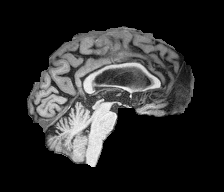
\includegraphics[height=#3, width=#3]{data/mri_sagittal.png}
		};

		\draw[fill=black] (input.north west) --
			($ (input.north west) + (0.5 * \mridepth, 0.5 * \mridepth) $) --
			($ (input.north east) + (0.5 * \mridepth, 0.5 * \mridepth) $) --
			(input.north east) -- cycle;
		\draw[fill=black] (input.north east) --
			($ (input.north east) + (0.5 * \mridepth, 0.5 * \mridepth) $) --
			($ (input.south east) + (0.5 * \mridepth, 0.5 * \mridepth) $) --
			(input.south east) -- cycle;
		\draw[] (input.north west) --
			($ (input.north west) - (0.5 * \mridepth, 0.5 * \mridepth) $) --
			($ (input.south west) - (0.5 * \mridepth, 0.5 * \mridepth) $) --
			(input.south west) -- cycle;
		\draw[] (input.north east) --
			($ (input.north east) - (0.5 * \mridepth, 0.5 * \mridepth) $) --
			($ (input.south east) - (0.5 * \mridepth, 0.5 * \mridepth) $) --
			(input.south east) -- cycle;
		\draw[] ($ (input.north west) - (0.5 * \mridepth, 0.5 * \mridepth) $) --
			($ (input.north east) - (0.5 * \mridepth, 0.5 * \mridepth) $);
		\draw[] ($ (input.south west) - (0.5 * \mridepth, 0.5 * \mridepth) $) --
			($ (input.south east) - (0.5 * \mridepth, 0.5 * \mridepth) $);
	}
	\newcommand{\convside}[6]{
		\def\sidex{#1}
		\def\sidey{#2}
		\def\sidewidth{#3}
		\def\sideheight{#4}
		\def\sidefillcolour{#5}
		\def\sidename{#6}

		\node[
			fill=\sidefillcolour,
			inner sep=0pt,
			outer sep=0pt,
			minimum width=\sidewidth,
			minimum height=\sideheight,
			draw=black
		] (\sidename) at (\sidex, \sidey) {};
	}

	\newcommand{\convtop}[4]{
		\def\topbase{#1}
		\def\topwidth{#2}
		\def\topheight{#3}
		\def\topfillcolour{#4}

		\draw[fill=\topfillcolour,draw=black] #1 --
			($ #1 + (#3, #3) $) --
			($ #1 + (#3+#2, #3) $) --
			($ #1 + (#2, 0) $);
	}

	\newcommand{\convfront}[3]{
		\def\frontbase{#1}
		\def\frontsize{#2}
		\def\frontfillcolour{#3}

		\draw[black, fill=\frontfillcolour] #1 --
			($ #1 + (1*#2, 1*#2) $) --
			($ #1 + (1*#2, 1*#2 - 2*#2) $) --
			($ #1 + (0, -2*#2) $);
	}

	\newcommand{\convchannel}[7]{
		\def\channelx{#1}
		\def\channely{#2}
		\def\channelnodedepth{#3}
		\def\channelnodesize{#4}
		\def\channelnodecount{#5}
		\def\channelcolour{#6}
		\def\includefront{#7}

		\def\huemin{20}
		\def\huemax{80}

		\pgfmathsetmacro{\iterations}{#5-1}
		\foreach \i in {0,...,\iterations} {
			\pgfmathsetmacro{\hue}{int(random(\huemin, \huemax))}
			\convside{#1}{#2+\i*-#4}{#3 cm}{#4 cm}{#6!\hue}{n\i0}

			\foreach \j in {0,...,\iterations} {
				\pgfmathsetmacro{\innerhue}{int(random(\huemin, \huemax))}
				\ifnum\j=0
					\pgfmathsetmacro{\innerhue}{\hue}
				\fi

				\ifnum\includefront=1
					\convfront{($ (n00.north east) + (0.5*\j*#4, 0.5*\j*#4 - \i*#4) $)}{0.5*#4}{#6!\innerhue}
				\fi

				\ifnum\i=0
					\convtop{($ (n\i0.north west) + (0.5*\j*#4, 0.5*\j*#4) $)}{#3}{0.5*#4}{#6!\innerhue}
				\fi
			}
		}
	}

	\newcommand{\convlayer}[7]{
		\def\layerx{#1}
		\def\layery{#2}
		\def\layernodedepth{#3}
		\def\layernodesize{#4}
		\def\layernodecount{#5}
		\def\layerdepth{#6}
		\def\layercolour{#7}

		\pgfmathsetmacro{\layeriterations}{\layerdepth-1}
		\foreach \i in {0,...,\layeriterations}{
			\pgfmathsetmacro{\x}{\layerx + \i * \layernodedepth}
			\pgfmathsetmacro{\islast}{\i == \layeriterations ? 1 : 0}
			\convchannel{\x}{\layery}{\layernodedepth}{\layernodesize}{\layernodecount}{\layercolour}{\islast}
		}
	}


	\newcommand{\modelarrow}[5]{
		\begin{scope}[transparency group, opacity=0.5]
			\draw[-stealth, line width=2pt, #3] #1 to [in=#4, out=#5] #2;
		\end{scope}
	}

	\newcommand{\cnnarrow}[3]{
		\modelarrow{#1}{#2}{#3}{180}{0}
	}

	\newcommand{\multitaskcnn}[5]{
		\def\xmin{#1}
		\def\ymin{#2}
		\def\nodedepth{#3}
		\def\nodesize{#4}
		\def\modelcolour{#5}

		\convlayer{#1 - 0.06 + 0.2}{#2 + 2.5 * #4}{#3}{#4}{12}{3}{\modelcolour}
		\cnnarrow{(#1 + 0.55, #2)}{(#1+1.5, #2)}{#5}

		\convlayer{#1 + 0.87 + 0.2}{#2 + 1.5 * #4}{#3}{#4}{8}{5}{\modelcolour}
		\cnnarrow{(#1 + 1.46, #2)}{(#1+2.2, #2)}{#5}

		\convlayer{#1 + 1.69 + 0.2}{#2 + 0.5 * #4}{#3}{#4}{4}{7}{\modelcolour}
		\cnnarrow{(#1 + 2.27, #2)}{(#1+2.9, #2)}{#5}

		\convlayer{#1 + 2.4 + 0.2}{#2 + 0}{#3}{#4}{2}{9}{\modelcolour}
		\cnnarrow{(#1 + 3.02, #2)}{(#1+3.46, #2)}{#5}

		\foreach \idx in {0, ..., 9} {
			\pgfmathsetmacro{\y}{#2 + 0.45 - \idx * 0.1}
			\pgfmathsetmacro{\hue}{int(random(20, 80))}
			\node[draw=black, fill=\modelcolour!\hue!white, minimum height=0.1cm, minimum width=0.1cm, inner sep=0pt] (b\idx) at (#1 + 3.12 + 0.4, \y) {};
		}

		\node[circle, minimum size=0.25cm, inner sep=0pt, draw=black] at (#1 + 4.5, #2-1) {};
		\node[circle, minimum size=0.25cm, inner sep=0pt, draw=black] at (#1 + 4.5, #2-0.6) {};
		\node[circle, minimum size=0.25cm, inner sep=0pt, draw=black] at (#1 + 4.5, #2-0.2) {};
		\node[circle, minimum size=0.25cm, inner sep=0pt, draw=black] at (#1 + 4.5, #2+0.2) {};
		\node[circle, minimum size=0.25cm, inner sep=0pt, draw=black] at (#1 + 4.5, #2+0.6) {};
		\node[circle, minimum size=0.25cm, inner sep=0pt, draw=black] at (#1 + 4.5, #2+1) {};

		\node[font=\scriptsize\linespread{0.9}\selectfont, align=left, anchor=west] at (#1 + 4.6, #2+1) {
			Brain age
		};
		\node[font=\scriptsize\linespread{0.9}\selectfont, align=left, anchor=west] at (#1 + 4.6, #2+0.6) {
			Sex
		};
		\node[font=\scriptsize\linespread{0.9}\selectfont, align=left, anchor=west] at (#1 + 4.6, #2+0.2) {
			Handedness
		};
		\node[font=\scriptsize\linespread{0.9}\selectfont, align=left, anchor=west] at (#1 + 4.6, #2-0.2) {
			BMI
		};
		\node[font=\scriptsize\linespread{0.9}\selectfont, align=left, anchor=west] at (#1 + 4.6, #2-0.6) {
			Neuroticism
		};
		\node[font=\scriptsize\linespread{0.9}\selectfont, align=left, anchor=west] at (#1 + 4.6, #2-1) {
			IQ
		};
		\cnnarrow{(#1 + 3.57, #2)}{(#1+4.37, #2+1)}{#5}
		\cnnarrow{(#1 + 3.57, #2)}{(#1+4.37, #2+0.6)}{#5}
		\cnnarrow{(#1 + 3.57, #2)}{(#1+4.37, #2+0.2)}{#5}
		\cnnarrow{(#1 + 3.57, #2)}{(#1+4.37, #2-0.2)}{#5}
		\cnnarrow{(#1 + 3.57, #2)}{(#1+4.37, #2-0.6)}{#5}
		\cnnarrow{(#1 + 3.57, #2)}{(#1+4.37, #2-1)}{#5}
	}

	\newcommand{\multitaskbox}{
		\begin{tikzpicture}
			\node[] at (-2.5, -2.5) {};
			\node[] at (6.7, 2.5) {};

			\inputside{-1.4}{0}{1cm}

			\cnnarrow{(input.east)}{($ (input.center) + (1.5, 0) $)}{black}

			\multitaskcnn{-0.43}{0}{0.044}{0.1}{black}
		\end{tikzpicture}
	}


	\newsavebox{\multitaskmodel}
	\sbox{\multitaskmodel}{
		\multitaskbox
	}

	\begin{frame}{Methods}
		\begin{tikzpicture}
			\node[] at (-5.25, -3.5) {};
			\node[] at (5.25, 3.5) {};

			\only<1>{
				\node[] at (0, 0) {
					\usebox{\datasetbox}
				};
			}
			\only<2>{
				\node[] at (0, 0) {
					\usebox{\multitaskmodel}
				};
			}
		\end{tikzpicture}
	\end{frame}

	\newcommand{\continuousplot}[6]{
		\def\fileprefix{#1}
		\def\title{#2}
		\def\axismin{#3}
		\def\axismax{#4}
		\def\pad{#5}

		\nextgroupplot[
			title=\scriptsize{#2},
			xmin=#3,
			xmax=#4,
			ymin=#3,
			ymax=#4,
			clip=false
		]
			\addplot[
				thick,
				red
			] coordinates {
				(#3, #3)
				(#4, #4)
			};
			\addplot[
				only marks,
				opacity=0.05,
				blue,
				mark size=1pt,
				%each nth point={10}
			] table [
				col sep=comma,
				x=true,
				y=predicted
			] {data/#1.csv};

			\node[font=\tiny\linespread{0.95}\selectfont\bfseries, text=red, anchor=south east, align=center] at (rel axis cs: 1.02, -0.02) {
				#6
			};
	}

	\newcommand{\binaryplot}[3]{
		\nextgroupplot[
			title=\scriptsize{#2}
		]
			\addplot[
				only marks,
				opacity=0.05,
				blue,
				mark size=1pt,
				%each nth point={10}
			] table [
				col sep=comma,
				x expr=\thisrow{true} + rand * 0.1 - 0.05,
				y=predicted
			] {data/#1.csv};
			\node[font=\tiny\linespread{0.95}\selectfont\bfseries, text=red, anchor=south, align=center] at (rel axis cs: 0.5, -0.02) {
				\underline{AUC}\\
				#3
			};
	}

	\newcommand{\multivalplot}{
		\begin{tikzpicture}
			\begin{groupplot}[
				group style={
					group name=toprow,
					group size=6 by 1,
					horizontal sep=0.1cm
				},
				xmajorticks=false,
				ymajorticks=false,
				height=3.1cm,
				width=3.1cm,
				title style={
					yshift=-0.2cm,
					text depth=0
				}
			]
				\continuousplot{multi_val_age}{Age}{0}{100}{0}{\underline{MAE}\\2.21}
				\binaryplot{multi_val_sex}{Sex}{0.99}
				\binaryplot{multi_val_handedness}{Handedness}{0.61}
				\continuousplot{multi_val_bmi}{BMI}{10}{50}{0}{\underline{MAE}\\2.38}
				\continuousplot{multi_val_fluid_intelligence}{Intelligence}{-5}{5}{0}{\underline{R}\\0.27}
				\continuousplot{multi_val_neuroticism}{Neuroticism}{-5}{5}{0}{\underline{R}\\0.17}
			\end{groupplot}
			\node[] at ($ (toprow c1r1.south) - (0, 0.15) $) {\tiny{Observed}};
			\node[rotate=90] at ($ (toprow c1r1.west) - (0.15, 0) $) {\tiny{Predicted}};
		\end{tikzpicture}
	}

	\newsavebox{\multivalbox}
	\sbox{\multivalbox}{
		\multivalplot
	}

	\newcommand{\multitestplot}{
		\begin{tikzpicture}
			\begin{groupplot}[
				group style={
					group size=6 by 1,
					horizontal sep=0.1cm
				},
				xmajorticks=false,
				ymajorticks=false,
				height=3.1cm,
				width=3.1cm
			]
				\continuousplot{multi_test_age}{}{0}{100}{0}{\underline{MAE}\\3.41}
				\binaryplot{multi_test_sex}{}{0.98}
				\binaryplot{multi_test_handedness}{}{0.48}{}
				\continuousplot{multi_test_bmi}{}{10}{50}{0}{\underline{MAE}\\1.95}
			\end{groupplot}
		\end{tikzpicture}
	}

	\newsavebox{\multitestbox}
	\sbox{\multitestbox}{
		\multitestplot
	}

	\newcommand{\regtestplot}{
		\begin{tikzpicture}
			\begin{groupplot}[
				group style={
					group size=6 by 1,
					horizontal sep=0.1cm
				},
				xmajorticks=false,
				ymajorticks=false,
				height=3.1cm,
				width=3.1cm
			]
				\continuousplot{reg_test_age}{}{0}{100}{0}{\underline{MAE}\\3.68}
			\end{groupplot}
		\end{tikzpicture}
	}

	\newsavebox{\regtestbox}
	\sbox{\regtestbox}{
		\regtestplot
	}

	\newcommand{\downstreamtrace}[4][solid]{
		\addplot[
			#3,
			thick,
			mark=*,
			draw opacity=0.75,
			fill opacity=0.75,
			mark size=4pt,
			#1
		] table [
			col sep=comma,
			x=size,
			y=#3_#4_mean
		] {#2};
	}
	\newcommand{\errortrace}[4][solid]{
		\addplot[
			#3,
			thick,
			mark=*,
			draw opacity=0.75,
			fill opacity=0.75,
			mark size=4pt,
			#1,
			error bars/.cd,
			y dir=both,   % Error bars in both directions
			y explicit
		] table [
			col sep=comma,
			x=size,
			y=#3_#4_mean,
			y error expr=\thisrow{#3_loss_sem} * 1.96
		] {#2};
	}

	\newcommand{\downstreamplot}[7]{
		\begin{tikzpicture}
			\begin{axis}[
				height=6.5cm,
				width=10cm,
				xtick=#5,
				ytick pos=#3,
				ylabel=#4,
				xlabel={Dataset size},
				xticklabel style={
				rotate=45,
				anchor=north east
				},
				xtick pos=bottom,
				ymajorgrids=true,
				ytick style={
					draw=none
				},
				clip=false,
				legend cell align=left,
				legend style={font=\footnotesize},
				legend pos=#7
			]

			\downstreamtrace{#1}{none}{#2}
			\downstreamtrace{#1}{finetune}{#2}
			\downstreamtrace{#1}{freeze}{#2}

			#6

			\end{axis}
		\end{tikzpicture}
	}

	\newcommand{\finetuneplot}[7]{
		\begin{tikzpicture}
			\begin{axis}[
				height=6.5cm,
				width=10cm,
				xtick=#5,
				ytick pos=#3,
				ylabel=#4,
				xlabel={Dataset size},
				xticklabel style={
				rotate=45,
				anchor=north east
				},
				xtick pos=bottom,
				ymajorgrids=true,
				ytick style={
					draw=none
				},
				clip=false,
				legend cell align=left,
				legend style={font=\footnotesize},
				legend pos=#7
			]

			\errortrace{#1}{finetune}{#2}

			#6

			\end{axis}
		\end{tikzpicture}
	}

	\newcommand{\heatmap}[3][]{
		\nextgroupplot[
			view={0}{90},
			colormap/temp,
			ymin=0,
			xmin=0,
			xmajorticks=false,
			ymajorticks=false,
			point meta min=-1,
			point meta max=1,
			#1,
			title=#3,
			title style={
				text depth=0,
				font=\bfseries,
				yshift=-0.2cm
			}
		]
			\addplot3 [
				surf,
				shader=flat corner, % Ensures flat shading between grid points
				mesh/rows=64,
				mesh/cols=64
			] table [
				col sep=comma,
				x=x,
				y=y,
				z=value,
			] {data/encodings/#2.csv};
	}

	\newsavebox{\encodings}
	\sbox{\encodings}{
		\begin{tikzpicture}
			\begin{groupplot}[
				group style={
					group size=2 by 1,
					horizontal sep=0.3cm
				},
				height=5.5cm,
				width=5.5cm
			]
				\heatmap{sfcn-reg}{Brain age}
				\heatmap[
					colorbar right,
					colorbar style={
						ylabel={Correlation},
						ytick={-1,0,1},
						tick style={draw=none},
						ylabel style={yshift=0.2cm}
					}
				]{sfcn-multi}{Multi-task}
			\end{groupplot}
		\end{tikzpicture}
	}

	\begin{frame}{Results}
		\begin{tikzpicture}
			\node[] at (-5.25, -3.5) {};
			\node[] at (5.25, 3.5) {};

			\only<1>{
				\node[anchor=west] (multival) at (-5, 1.75) {
					\usebox{\multivalbox}
				};
				\node[anchor=south, rotate=90, font=\scriptsize\linespread{0.95}\selectfont\bfseries, align=center] at ($ (multival.west) - (-0.35, 0.05) $) {
					Multi-task\\(validation)
				};
				\node[anchor=west] (multitest) at (-4.655, 0) {
					\usebox{\multitestbox}
				};
				\node[anchor=south, rotate=90, font=\scriptsize\linespread{0.95}\selectfont\bfseries, align=center] at ($ (multitest.west) - (0, 0.2) $) {
					Multi-task\\(test)
				};
				\node[anchor=west] (regtest) at (-4.655, -1.65) {
					\usebox{\regtestbox}
				};
				\node[anchor=south, rotate=90, font=\scriptsize\linespread{0.95}\selectfont\bfseries, align=center] at ($ (regtest.west) - (0, 0.2) $) {
					Brain age\\(test)
				};
			}
			\only<2>{
				\node[] at (0, 0) {
					\usebox{\encodings}
				};
			}
			\only<3>{
				\node[] at (0, 0) {
					\downstreamplot{data/downstream/age.csv}{loss}{left}{Relative Absolute Error}{{100, 250, 500, 1000, 2500}}{
						\downstreamtrace{data/downstream/age.csv}{pretrained}{loss}

						\addlegendentry{Baseline}
						\addlegendentry{Finetuned}
						\addlegendentry{Frozen}
						\addlegendentry{Transferred}
					}{north east}
				};
			}
			\only<4>{
				\node[text width=10cm] at (0, 0.5) {
					\begin{itemize}
						\item Each entry is the average over 100 bootstrapped training samples of size $n$
						\begin{itemize}
							\item Additional 20\% for validation and 20\% for testing
							\item 9 models with different hyperparameters are fit, the best is selected based on validation performance
						\end{itemize}
						\item A model trained from scratch (baseline), and three using different transfer learning strategies
						\begin{itemize}
							\item Transferred: The pretrained model is directly applied
							\item Frozen: The pretrained model is retrained while freezing everything but the final layer
							\item Finetuned: The pretrained model is used for initialization, then fully retrained
						\end{itemize}
					\end{itemize}
				};
			}
			\only<5>{
				\node[] at (0, 0) {
					\downstreamplot{data/downstream/age_top.csv}{loss}{left}{Relative Absolute Error}{{100, 200, 300, 400, 500}}{
						\downstreamtrace{data/downstream/age_top.csv}{pretrained}{loss}

						\addlegendentry{Baseline}
						\addlegendentry{Finetuned}
						\addlegendentry{Frozen}
						\addlegendentry{Transferred}
					}{north east}
				};
			}
			\only<6>{
				\node[] at (0, 0) {
					\downstreamplot{data/downstream/ad.csv}{loss}{left}{Relative Absolute Error}{{100, 200, 300, 400, 500}}{
						\downstreamtrace[densely dotted]{data/downstream/reg.csv}{finetune}{loss}
						\downstreamtrace{data/downstream/linear_ad.csv}{linear}{loss}

						\addlegendentry{Baseline}
						\addlegendentry{Finetuned}
						\addlegendentry{Frozen}
						\addlegendentry{Brain age}
						\addlegendentry{Linear}
					}{south east}
				};
			}
			\only<7>{
				\node[] at (0, 0) {
					\downstreamplot{data/downstream/scz.csv}{loss}{left}{Relative Absolute Error}{{100, 200, 300, 400, 500}}{
						\downstreamtrace{data/downstream/linear_scz.csv}{linear}{loss}

						\addlegendentry{Baseline}
						\addlegendentry{Finetuned}
						\addlegendentry{Frozen}
						\addlegendentry{Linear}
					}{north west}
				};
			}
			\only<8>{
				\node[] at (0, 0) {
					\finetuneplot{data/downstream/asd.csv}{loss}{left}{Relative Absolute Error}{{100, 450, 800, 1150, 1500}}{
						\errortrace{data/downstream/linear_asd.csv}{linear}{loss}

						\addlegendentry{Finetuned}
						\addlegendentry{Linear}
					}{north west}
				};
			}
			\only<9>{
				\node[text width=10cm, align=flush left] at (0, 0) {
					Why does the deep learning model not behave asymptotically?
					\begin{itemize}
						\item It shouldn't (bad luck?)
						\item Double descent? (\emoji{crossed-fingers})
						\item Some property of the data? (heterogeneity?)
						\item Some property of the model? (too simple?)
						\item \textbf{Some property of the procedure?}
					\end{itemize}
				};
			}

		\end{tikzpicture}
	\end{frame}
\end{document}
